\section{Strutture fisiche e accesso ai dati}

Per comprendere il funzionamento interno di un DBMS è necessario analizzare come i dati vengono effettivamente memorizzati e gestiti a livello fisico.

Una base di dati risiede in memoria secondaria per due motivi fondamentali. 
In primo luogo, per una questione di \textbf{dimensione}: le basi di dati sono generalmente molto grandi e non possono essere contenute interamente in memoria centrale. 
In secondo luogo, per garantire la \textbf{persistenza}: i dati devono sopravvivere all'esecuzione dei programmi e agli spegnimenti del sistema. 
A differenza della memoria centrale, che è volatile, la memoria secondaria consente di conservare le informazioni in modo permanente nel tempo.

La memoria secondaria presenta però alcune caratteristiche che influenzano direttamente il modo in cui i dati vengono gestiti. 
Essa non è direttamente accessibile dai programmi e i dati sono organizzati in \textbf{blocchi} (o pagine). 
Di conseguenza, non è possibile leggere una singola informazione in modo puntuale: quando si accede a un dato, è necessario caricare in memoria centrale l'intero blocco che lo contiene. 
Le uniche operazioni possibili sulla memoria secondaria sono quindi la \textbf{lettura} e la \textbf{scrittura} di blocchi.

Un aspetto cruciale è che tali operazioni hanno un costo molto elevato rispetto agli accessi alla memoria centrale, con una differenza di diversi ordini di grandezza. 
Per questo motivo, nella valutazione delle prestazioni di un DBMS non si considera il numero di operazioni di calcolo, ma il \textbf{numero di accessi alla memoria secondaria}, che rappresenta il vero collo di bottiglia del sistema.

Per ridurre il numero di accessi al disco interviene il \textbf{gestore del buffer} (buffer manager), che ha il compito di gestire la memoria centrale. 
Questo modulo mantiene in RAM i blocchi più utilizzati, evitando accessi ripetuti alla memoria secondaria. 
Quando un blocco non è presente in memoria, il buffer manager richiede il caricamento dal disco; analogamente, quando un blocco viene modificato, si occupa della sua scrittura in memoria secondaria.

Il \textbf{gestore della memoria secondaria} è invece responsabile dell'accesso fisico ai dati. 
Esso gestisce i file del database e si occupa delle operazioni di lettura e scrittura dei blocchi, interagendo direttamente con il file system del sistema operativo. 
In questo contesto, il gestore del buffer e quello della memoria secondaria collaborano strettamente: il primo richiede i blocchi necessari, mentre il secondo li recupera dal disco.

Infine, il \textbf{gestore dell'affidabilità} interviene per garantire la correttezza del sistema anche in presenza di guasti. 
Questo modulo mantiene un log delle operazioni eseguite e consente il ripristino dello stato corretto del database tramite operazioni di \textit{redo} e \textit{undo}, assicurando la persistenza delle transazioni completate.
L'interazione tra memoria secondaria e memoria centrale avviene tramite il \textbf{gestore del buffer}, che si occupa di trasferire i dati dal disco alla RAM sotto forma di blocchi.

In particolare, il buffer manager carica uno o più blocchi dalla memoria secondaria in \textbf{pagine} della memoria centrale. 
Sebbene non vi sia una corrispondenza perfetta, si assume generalmente che una pagina in memoria centrale corrisponda a un blocco in memoria secondaria.

Il buffer rappresenta quindi un'area di memoria centrale condivisa tra più applicazioni, il cui obiettivo è ridurre il numero di accessi alla memoria secondaria.

Il gestore del buffer ha il compito di:
\begin{itemize}
	\item caricare i blocchi dalla memoria secondaria alla memoria centrale;
	\item restituire riferimenti (puntatori) ai dati richiesti;
	\item scrivere i blocchi modificati dalla memoria centrale al disco.
\end{itemize}

Per ottimizzare le prestazioni, il buffer manager adotta diverse \textbf{politiche di gestione della memoria}, che riguardano sia le operazioni di lettura sia quelle di scrittura.

Nel caso della \textbf{lettura di un blocco}, si distinguono due situazioni:
\begin{itemize}
	\item se il blocco è già presente nel buffer (\textit{buffer hit}), non viene effettuato alcun accesso alla memoria secondaria e viene restituito direttamente il riferimento alla pagina in memoria centrale;
	\item se il blocco non è presente (\textit{buffer miss}), esso viene caricato dal disco e successivamente reso disponibile.
\end{itemize}

Nel caso della \textbf{scrittura}, il DBMS può adottare una strategia di \textbf{scrittura differita} (\textit{delayed write}): il blocco modificato viene aggiornato inizialmente solo in memoria centrale e la scrittura su disco viene posticipata. 
Questa scelta migliora le prestazioni riducendo il numero di operazioni di I/O, ma introduce il rischio di perdita dei dati in caso di guasto. 
Per questo motivo interviene il \textbf{gestore dell'affidabilità}, che tramite il log consente di ripristinare le informazioni corrette.

Le politiche di gestione del buffer si basano sul \textbf{principio di località}, secondo cui i dati recentemente utilizzati hanno un'alta probabilità di essere riutilizzati nel breve periodo.

Un'importante osservazione empirica è la cosiddetta \textbf{regola dell'80/20}: circa il 20\% dei dati è responsabile dell'80\% degli accessi. 
Questo implica che, mantenendo in memoria centrale una piccola parte dei dati più frequentemente utilizzati, è possibile ottenere un notevole miglioramento delle prestazioni.

Per questo motivo, politiche semplici come la LIFO (Last In First Out) risultano inefficaci, poiché non tengono conto del principio di località. 
Al contrario, strategie più evolute (come LRU, Least Recently Used) privilegiano il mantenimento in memoria dei dati utilizzati più di recente.
\subsection{Rappresentazione logica del buffer}

Il contenuto del buffer può essere rappresentato in maniera logica come una \textbf{matrice di pagine}, tutte aventi la stessa dimensione.

Ogni pagina del buffer può contenere un blocco $B$ proveniente dalla memoria secondaria. 
Si assume quindi, in prima approssimazione, una corrispondenza tra pagine in memoria centrale e blocchi in memoria secondaria.

Per ogni pagina del buffer che contiene un blocco, vengono mantenute due importanti \textbf{variabili di stato}:

\begin{itemize}
	\item un \textbf{contatore} $i$, che indica quante transazioni stanno attualmente utilizzando quella pagina;
	
	\item un \textbf{bit di stato} $j$ (dirty bit), che indica se la pagina è stata modificata:
	\begin{itemize}
		\item $j = 1$ se la pagina è stata modificata rispetto al contenuto in memoria secondaria;
		\item $j = 0$ se la pagina è identica a quella presente su disco.
	\end{itemize}
\end{itemize}

Il contatore $i$ è fondamentale per la gestione della concorrenza, in quanto impedisce la rimozione di una pagina ancora in uso da parte di una o più transazioni.

Il bit di stato $j$ è invece essenziale per la gestione delle scritture: una pagina modificata deve essere salvata su memoria secondaria prima di essere eventualmente rimossa dal buffer.

In Figura~\ref{fig:image188} è mostrata una possibile rappresentazione del buffer come matrice di pagine, in cui alcune pagine contengono blocchi della memoria secondaria e sono associate ai rispettivi stati.

\begin{figure}[H]
	\centering
	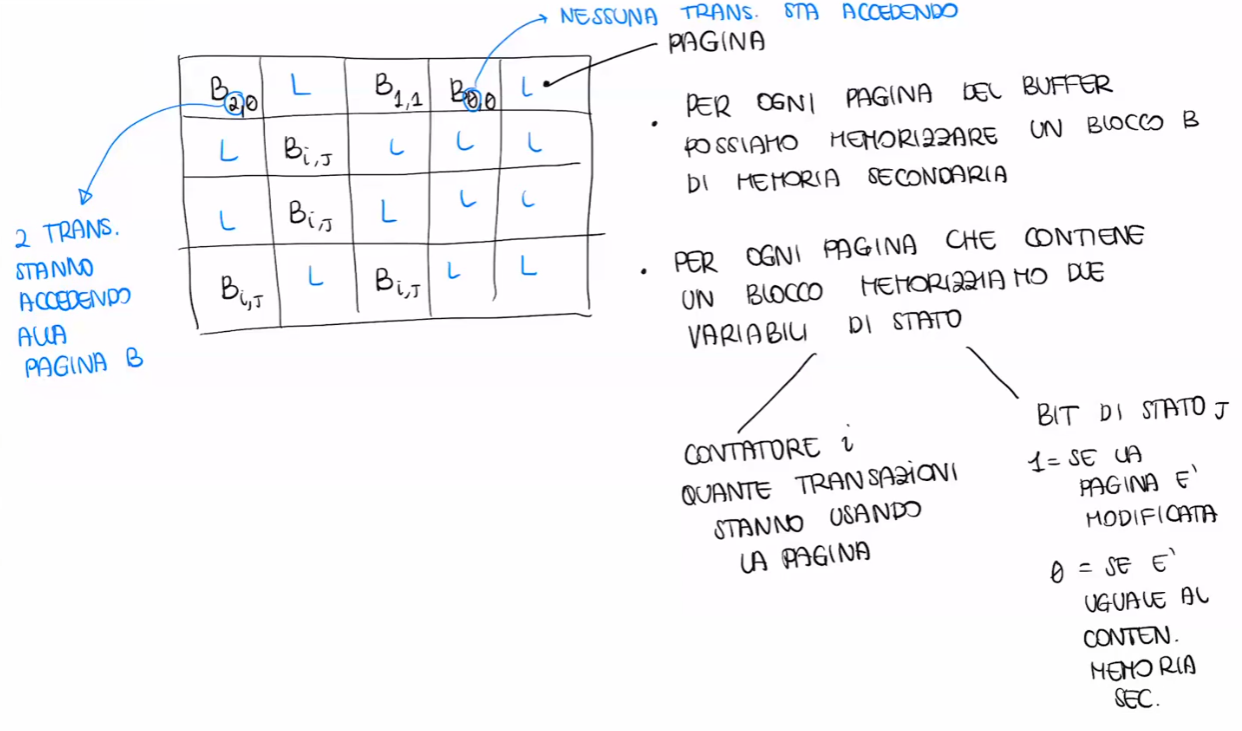
\includegraphics[width=1\linewidth]{image188}
	\caption{Rappresentazione logica del buffer}
	\label{fig:image188}
\end{figure}
\subsection{Primitive del gestore del buffer}

Il gestore del buffer mette a disposizione un insieme di primitive utilizzate principalmente dal gestore dei metodi di accesso per richiedere e gestire i blocchi in memoria centrale.

\begin{enumerate}
	\item \textbf{FIX}
	
	La primitiva FIX viene utilizzata per richiedere l'accesso a un blocco della memoria secondaria. 
	Essa restituisce un puntatore alla pagina del buffer che contiene il blocco richiesto.
	
	Il comportamento può essere descritto nei seguenti casi:
	
	\begin{itemize}
		\item \textbf{Caso 1: blocco già presente nel buffer (buffer hit)} \\
		Se il blocco è già caricato, il sistema restituisce semplicemente il puntatore alla pagina corrispondente.
		
		\item \textbf{Caso 2: blocco non presente (buffer miss)} \\
		Il sistema deve caricare il blocco in una pagina del buffer.
		
		\begin{itemize}
			\item Se esiste una \textbf{pagina libera} (indicata, ad esempio, con etichetta $L$ oppure con contatore $i = 0$), essa viene utilizzata.
			
			\item Se non esistono pagine libere, è necessario scegliere una pagina da sostituire secondo una politica di rimpiazzamento, come:
			\begin{itemize}
				\item \textbf{LRU} (Least Recently Used): rimuove la pagina meno recentemente utilizzata;
				\item \textbf{FIFO} (First In First Out): rimuove la pagina caricata da più tempo.
			\end{itemize}
		\end{itemize}
		
		Prima di riutilizzare una pagina, si verifica il valore del \textbf{dirty bit} $j$:
		\begin{itemize}
			\item se $j = 1$, la pagina deve essere scritta su disco tramite la primitiva \textit{FLUSH};
			\item se $j = 0$, può essere riutilizzata immediatamente.
		\end{itemize}
		
		\item \textbf{Caso 3: Gestione in assenza di pagine disponibili} \\
		Se tutte le pagine sono in uso (cioè con contatore $i > 0$), il DBMS può adottare due strategie:
		
		\begin{itemize}
			\item \textbf{NO-STEAL}: la transazione viene sospesa finché non si libera una pagina;
			\item \textbf{STEAL}: il sistema può sottrarre una pagina a un'altra transazione, anche se ancora in uso.
		\end{itemize}
	\end{itemize}
	
	Dopo il caricamento del blocco, il contatore $i$ della pagina viene incrementato.
	
	\item \textbf{UNFIX}
	
	La primitiva UNFIX indica che una transazione ha terminato di utilizzare un blocco. 
	Di conseguenza, il contatore $i$ associato alla pagina viene decrementato.
	
	\item \textbf{SETDIRTY}
	
	Questa primitiva viene utilizzata quando una transazione modifica il contenuto di una pagina. 
	Il dirty bit $j$ viene posto a 1, indicando che la copia in memoria centrale è diversa da quella in memoria secondaria.
	
	\item \textbf{FLUSH}
	
	La primitiva FLUSH consente di scrivere su memoria secondaria una pagina modificata. 
	Questa operazione può avvenire in modo asincrono ed è utilizzata dal gestore del buffer per liberare spazio.
	
	Al termine dell'operazione, il dirty bit $j$ viene posto a 0.
	
	\item \textbf{FORCE}
	
	La primitiva FORCE è una variante della FLUSH, utilizzata per garantire la scrittura immediata di una pagina su memoria secondaria. 
	Essa è tipicamente richiesta dal gestore dell'affidabilità per assicurare la persistenza dei dati.
	
	Anche in questo caso, al termine dell'operazione il dirty bit $j$ viene posto a 0.
\end{enumerate}
